\section{Objetivos Y Estructura}
\label{Objetivos Y Estructura}

    Diseñar y construir Colivi constituye el objetivo principal de este proyecto, ofreciendo una plataforma web que da respuesta a la búsqueda de habitaciones y a la organización interna en pisos de estudiantes. La aplicación acompaña a los usuarios durante todo el ciclo: conecta al arrendatario con el propietario durante la reserva y estructura el reparto de tareas domésticas una vez comenzada la convivencia.
    
    La consecución de esta meta global se desglosa en los siguientes objetivos específicos:

\begin{enumerate}
    \item Implementar un módulo de seguridad para registro e inicio de sesión mediante tókenes JWT, distinguiendo perfiles de inquilino y propietario.
    \item Habilitar la edición del perfil de usuario con datos de contacto, preferencias y hábitos de convivencia.
    \item Desarrollar un buscador de habitaciones con filtrado por localización geográfica, precio mensual, equipamiento y normas de estancia.
    \item Construir un canal de mensajería contextual asociado a cada anuncio que permita plantear dudas al anfitrión sin exigir una reserva previa.
    \item Programar el ciclo de vida de las solicitudes de reserva con control estricto de estados y depósitos de fianza.
    \item Diseñar un planificador gamificado de tareas domésticas basado en turnos rotativos (\emph{Round-Robin}), tabla de puntuaciones y posibilidad de rescate entre compañeros.
    \item Disponer un registro inmutable de auditoría para monitorizar acciones clave dentro del hogar, como la realización de limpiezas o la incorporación de nuevos miembros.
    \item Integrar un asistente inteligente fundamentado en el protocolo \emph{Model Context Protocol} (MCP) que consulte turnos, resuma actividad o filtre anuncios sin modificar la base de datos.
\end{enumerate}

    La arquitectura global del sistema (reflejada en la figura~\ref{fig:estructura_tecnica_colivi}) distribuye sus responsabilidades en cuatro capas desacopladas: el cliente web, el servidor central de aplicaciones, el microservicio de soporte inteligente y el motor de persistencia relacional.

    El cliente web interactúa directamente con el usuario mediante una interfaz reactiva construida con React, TypeScript y Tailwind CSS. Vite actúa como empaquetador para optimizar los tiempos de recarga durante el desarrollo y minimizar el tamaño del paquete final en producción. La sincronización de datos asíncronos recae en TanStack Query, aplicando una estrategia de sondeo controlado (\emph{Smart Polling}) que refresca los mensajes y las tareas únicamente mientras la pestaña del navegador permanece en primer plano, evitando la sobrecarga de conexiones persistentes innecesarias.

    El backend principal se ejecuta sobre la máquina virtual de Java 21 utilizando Spring Boot 3. Este servidor expone una API REST dividida en módulos de dominio bajo principios SOLID. Procesa reglas de negocio críticas: el reparto equitativo de turnos de limpieza, la desvinculación automática de reservas mediante eventos internos de dominio (@EventListener) y la contención de colisiones concurrentes mediante bloqueos pesimistas en las tablas afectadas. Asimismo, se apoya en Spring AI para consultar modelos de lenguaje remotos a través de la API de Groq, devolviendo respuestas formateadas en JSON estricto.

    Un microservicio complementario desarrollado en Node.js y TypeScript expone un servidor MCP oficial mediante \emph{Server-Sent Events} (SSE). Este servicio declara herramientas de inspección de anuncios, consulta de estado de tareas y cola de moderación. Cada conexión hereda el token JWT emitido por el backend, imponiendo un aislamiento estricto de solo lectura para evitar que la inteligencia artificial altere tablas de forma directa.

    La persistencia de datos reside en un clúster relacional de PostgreSQL. Mediante JPA e Hibernate se gestionan las entidades de usuarios, publicaciones, conversaciones, trazas de auditoría y turnos periódicos. Se aplicaron índices compuestos y restricciones de unicidad para descartar registros duplicados y mantener la integridad referencial en todo momento.

\begin{figure}[htbp]
    \centering
    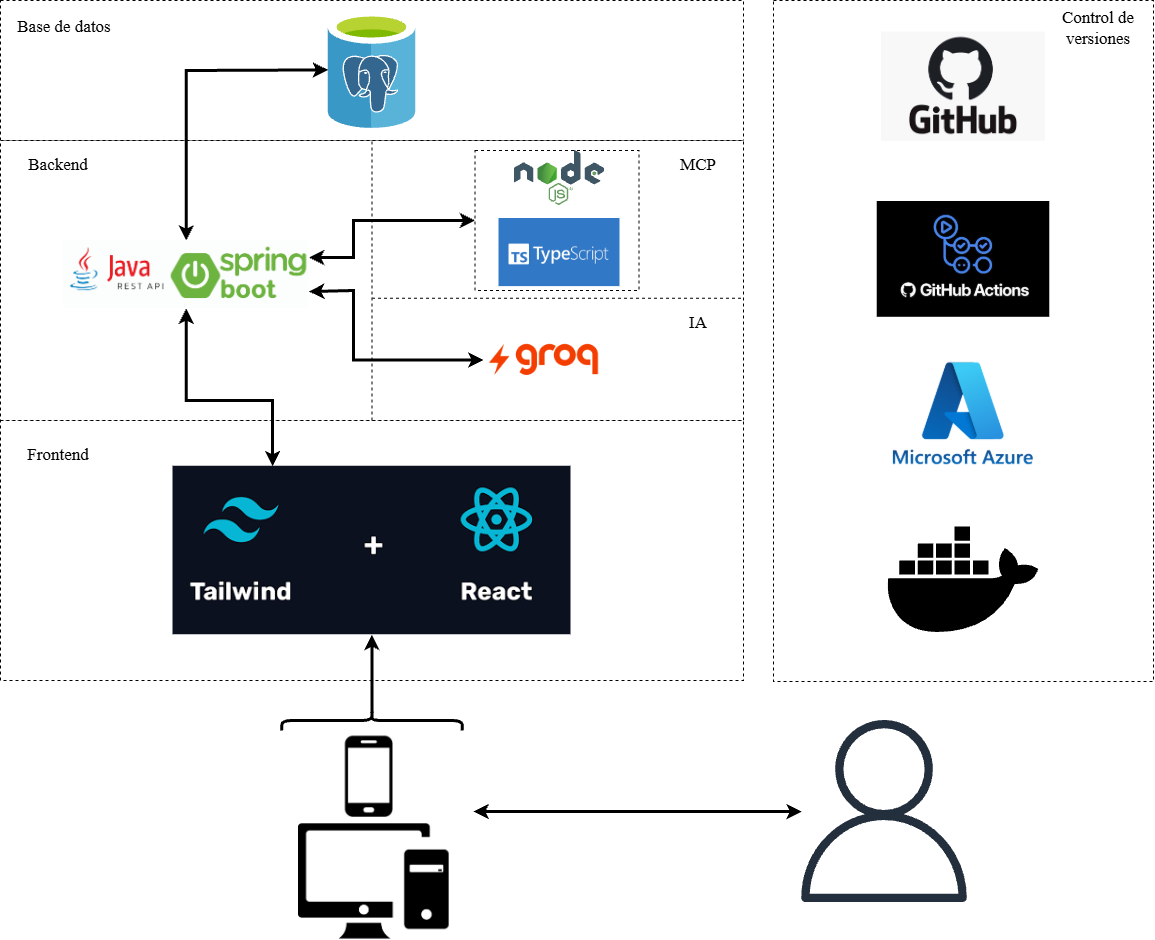
\includegraphics[width=0.85\textwidth]{Introduccion/img/Figura1.1.png}
    \caption{Estructura técnica global y arquitectura de la plataforma Colivi}
    \label{fig:estructura_tecnica_colivi}
\end{figure}